\chapter{Implementation}
\label{chap:impl}
In this chapter we give a formal overview of the system architecture,
some of the core classes and the most important
features of LDBN~- the different normalization algorithms and the user interface. 
In addition, we give an overview
of some key aspects of the server side implementation and communication
between server and client. At the end of the chapter we go over some
security issues and how LDBN deals with those. 

\section{System Architecture}
Figure~\ref{fig:sysarch} illustrates the architecture of LDBN. 
As can be seen, the architecture is decentralized. The client side implements 
all of the tutoring functions and the server side is used only for storing data.
As it was mentioned earlier, such a decentralized architecture ensures fewer HTTP requests to
the server, which in a single-thread environment as JavaScript means faster 
responses of the UI to user inputs. The architecture also reduces the server load,
which implies that the server can handle more users.

\begin{figure}[h]
	\begin{center}
		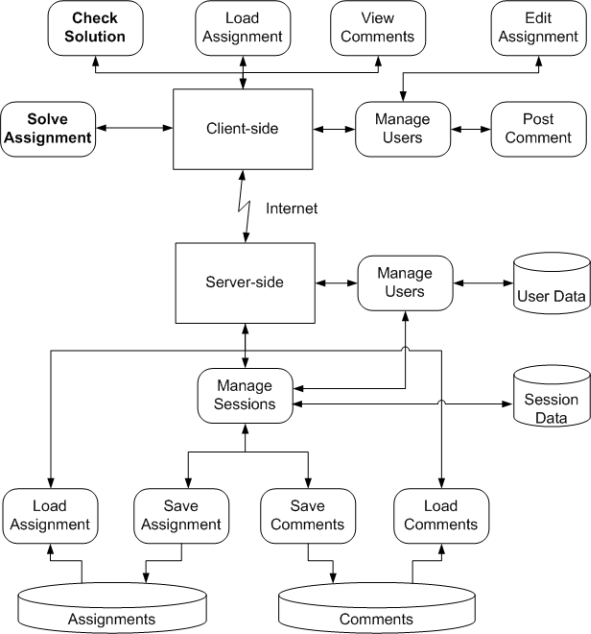
\includegraphics[width=0.85\textwidth]{./img/architecture01a.png}
		\caption{LDBN - System Architecture}
		\label{fig:sysarch}
	\end{center}
\end{figure}

It should be noted that the functions in the diagram represent many classes and 
static methods, which all serve the same purpose/function. We do not 
discuss all 
of the functions in detail, because most of them are straightforward and 
self-explanatory. 

\subsubsection{The Client-Side Functions}

\begin{description}
	\item[The Solve Assignment] function is used for generating a sample solution to 
		a given assignment, and presenting it to the user. As we mentioned in 
		Section~\ref{sec:introldbn}, an assignment consist of a relation schema in universal-relation form (URF).
	\item[The Check Solution] function, as the name suggests, performs series of checks to 
		test the correctness of the given solution. A solution to an assignment consists 
		of a decomposition of the schema from URF into 2NF, 3NF and BCNF. In addition,
		the user must identify one of the candidate keys of each new relation
    in the decomposition as the primary key of that relation.
	\item[The Load Assignment] function presents a list of all assignments, which are 
		stored in the database, to the user, and it can load new assignment from that list
		in the UI.
	\item[The Manage Users] function allows unregistered users to create new accounts 
		and registered users to login with their password and user-name. 
	\item[The Post Comment] function gives registered users the ability to comment an assignment, 
		thus be able to communicate with all other users.
	\item[The View Comments] function displays comments for each assignment, posted by registered users.
	\item[The Edit Assignment] function provides registered users with the 
		ability to create, edit, save, export and import assignments. 
\end{description}

As we can see from Figure~\ref{fig:sysarch} the functions \textit{Post Comments} 
and \textit{Edit Assignments} do not directly communicate with the server side, but rather 
communication goes first trough the \textit{Manage Users} function. This is done in order 
to ensure that the users are properly logged onto the system before attempting 
to use those functions. We will refer to functions which require users to login as restricted. 

The functions \textit{Solve Assignment} and \textit{Check Solution} are definitely the most 
important functions of LDBN, therefore we illustrate how they perform their tasks
in more detail in Section~\ref{sec:keyfunctions}. 

\subsubsection{The Server Side Functions}
Most of the functions on the server side are used as communication links (CL) for the
functions on the client side to the database. This means they retrieve/store data from/in the 
database, and then convert the data to an XML string and send it back to the client side
functions. 

\begin{description}
	\item[The Load Assignment] function is the CL for the \textit{Load Assignment} function on the 
		client side.
	\item[The Load Comments] function is the CL for the \textit{View Comments} function.
	\item[The Manage Sessions] function ensures that the data are coming from a registered user.
		It is also responsible for creating a new session, and terminating an existing one. Furthermore,
		each session has a unique ID, which is generated and sent back to the user 
		when he/she has logged in. This ID is stored in the \textit{Session Data} and it is used for
		authenticating the user in order for him/her to obtain access to restricted functions.
	\item[The Manage Users] function is the CL of the \textit{Manage Users} on the client side.
		It is responsible 
		for inserting new users into the database and for modifying existing data such as 
		user-name, password and email.
		It uses the \textit{Manage Sessions} function in order to ensure that a
		user is always logged in, before he/she attempts to change any user data.  
	\item[The Save Assignment] function is the CL for the \textit{Edit Assignment} function on the client side. 
		It is a restricted function, thus it uses the \textit{Manage Sessions} function. 
	\item[The Save Comment] function is CL for the \textit{Post Comment} function on the client side, it is 
		a restricted function as well.
\end{description} 

\section{Core Package of LDBN}
\label{sec:corepk}
Before moving to Section~\ref{sec:keyfunctions}, where we discuss the most important functions of 
LDBN namely the \textit{Solve Assignment} and the \textit{Check Solution} functions, 
we present the core package of LDBN. This package contains the foundation 
classes, on which both of the functions depend, therefore it is an essential 
part of LDBN. 

A very important part of LDBN is the representation of sets of attributes, since all 
data items in a database schema are based on sets of attributes. Therefore we developed an
efficient data structure called \verb=AttributeSet=, which holds a (sub)set of attributes of a relation.  
Before going into more detail, we present the different data items in LDBN. 
We refer to data items as items necessary to describe a database schema.  
The three fundamental items in our implementation are relations, FDs, and keys. Furthermore,
we are interested only in candidate keys and primary keys of a relation, not in not in non-minimal superkeys.
Figure~\ref{fig:relexample} illustrates
an (abstract) example of those data items and their structure in our system. 

%\begin{figure}[h]
%  \begin{center}
%    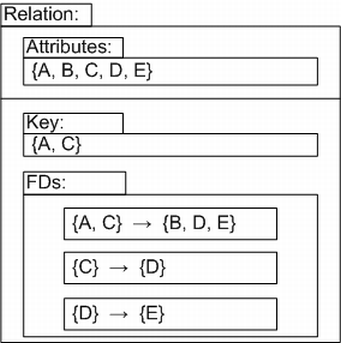
\includegraphics[scale=0.4]{./img/relation-example01a.png}
%    \caption{Example of a Relation}
%    \label{fig:relexample}
%  \end{center}
%\end{figure}

\begin{figure}[h]
  \centering
  \subfigure[Standard Representation]{
    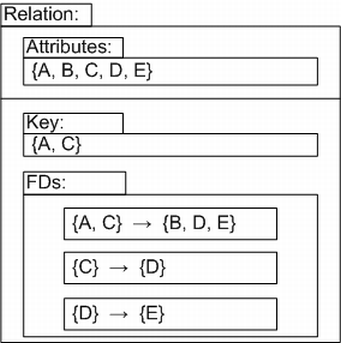
\includegraphics[scale=0.4]{./img/relation-example01a.png}
    \label{fig:relexample}
  }
  \subfigure[Representaion with Respect to AttributeSet]{
    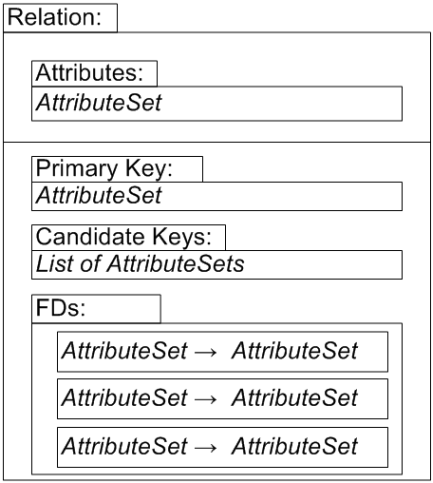
\includegraphics[scale=0.4]{./img/relation-example02a.png}
    \label{fig:relexample2}
  }
\caption{Example of a Relation Representation in LDBN}
\end{figure}

As can be seen, the most important data item is the relation, since
it holds the other two data items. This suggests itself, because FDs and keys have meaningful
interpretation only in combination with a relation. Furthermore, a key is a subset of 
the relation's attributes.
Each relation have a set of candidate keys and one primary key, which is an element form that set. 
Moreover, each relation is assigned a set of FDs. On the other hand, 
each FD consists of two subsets of
the relation's attributes, these represent the left-hand side (LHS) and the 
right-hand side (RHS) of an FD. Finally, a database schema or a decomposition of
a database schema can be described as a set of relations.

As the reader may have noticed, each data item consists of attributes and/or other
data items. Therefore we can use only our data structure \verb=AttributeSet=
in order to describe how the different data items are constructed. 
Figure~\ref{fig:relexample2} shows the same relation as in Figure~\ref{fig:relexample} with
respect to the instances of the \verb=AttributeSet= necessary to construct the different
data items.

%\begin{figure}[h]
%  \begin{center}
%    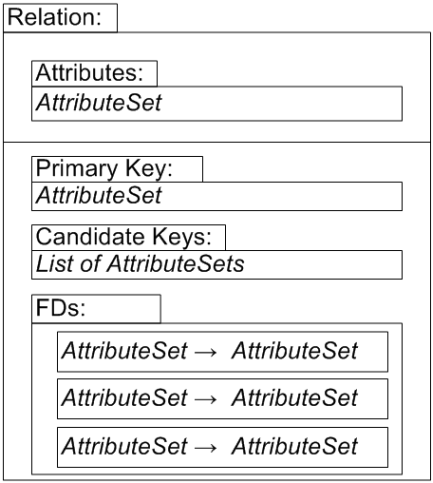
\includegraphics[scale=0.4]{./img/relation-example02a.png}
%    \caption{Example of a Relation with respect to AttributeSet}
%    \label{fig:relexample2}
%  \end{center}
%\end{figure}

As can be seen a (primary) key is simply an instance of \verb=AttributeSet=. The candidate keys
are represented as a list of instances of \verb=AttributeSet=. An FD is constructed from
two instances of \verb=AttributeSet=, one for the LHS and one for the RHS. And finally,
a relation is a composition of an instance of  \verb=AttributeSet= for representing
the relation's attributes, a primary key, a list of candidate keys and a list of FDs. 

Here follows a description of the implementation of the \verb=AttributeSet= data structure. 
In the early stages of the implementation of LDBN the \verb=AttributeSet=
was simply an array of strings. However, this has proven to be very
inefficient even for trivial operations such as comparison or union of two sets. This could 
lead to efficiency problems with
bigger assignments, since set operations are used quite often due to the exponential
complexity of many algorithms in LDBN. 
The solution was to use a bit-vector (boolean array) representation of sets of attributes. 
The data structure is described 
in~\cite[Section 4.3]{AhoHU83dsabook}. 
A set is represented by a bit-vector in which the $i^{th}$ bit is true if $i$ is an element of the set. In our
implementation every attribute of a relation is assigned a bit index. This is
done when an assignment is loaded and
we know all the possible attributes. Furthermore, we use an integer variable for representing
the bit-vector. This has the disadvantage that
assignments can contain only up to 32 attributes, but exceeding 32 attribute 
is highly unlikely to happen in an educational software. In addition, 
it would be an easy extension to support any multiple
of 32 bits simply by using an array of integers and applying the
operations element by element. On the other side, the 
advantages of the bit-vector representation are of much greater value, 
as set operations, which are used quite 
often, are performed in constant time, since we only use bitwise operators. The following 
table illustrates how exactly different set operations such as 
UNION, INTERSECTION, and DIFFERENCE are performed.
 
\begin{center}
\begin{tabular}[h]{|l|l|}
\hline
Set Operation & Bitwise Operator \\
\hline
\hline
UNION        & bit-vector$_1$  OR  bit-vector$_2$ \\
INTERSECTION & bit-vector$_1$ AND  bit-vector$_2$ \\
DIFFERENCE   & bit-vector$_1$ AND (NOT bit-vector$_2$) \\
\hline
\end{tabular}
\end{center}

In the following we would like to present other key aspects of the Core package. For reference we 
use Figure~\ref{fig:coreuml}, which shows an UML class diagram of the most important 
classes and methods of the package. We already discussed most of the classes like the \verb=AttributeSet=,
the \verb=Key=, the \verb=FD= and the \verb=Relation= classes. Now we are going to present the  
\verb=AttributeNameTable= class. Every \verb=AttributeSet= object has an associated domain name space called 
\verb=AttributeNameTable=. It contains a map, such that the string name of an attribute is mapped to its 
integer representation. In this way, information is never lost. 
Furthermore, the \verb=AttributeNameTable=
class uses the event listener (also known as event handler) design pattern, 
as a result of which classes implementing 
the \verb=AttributeNameTableListner= interface can update their content,
whenever changes in the \verb=AttributeNameTable= occur. This is used by instances of the 
\verb=AttributeSet= class, but also by some UI classes, which are not shown in the diagram. 

The \verb=Algorithm= class contains all of the normalization algorithms used by LDBN to perform 
the \textit{Solve Assignment} and \textit{Check Solution} functions. The algorithms are implemented 
as static functions. Many of them have exponential complexity in the worst
case. Therefore a lot of the produced output is being cached. This increases the
memory usage, but it could make the application respond much quicker, which
in our opinion is more important for the user. The normalization algorithms are very important 
part of LDBN. We present them in detail in the next section. 

\begin{figure}[htbp]
  \begin{center}
\hspace*{-0.5cm}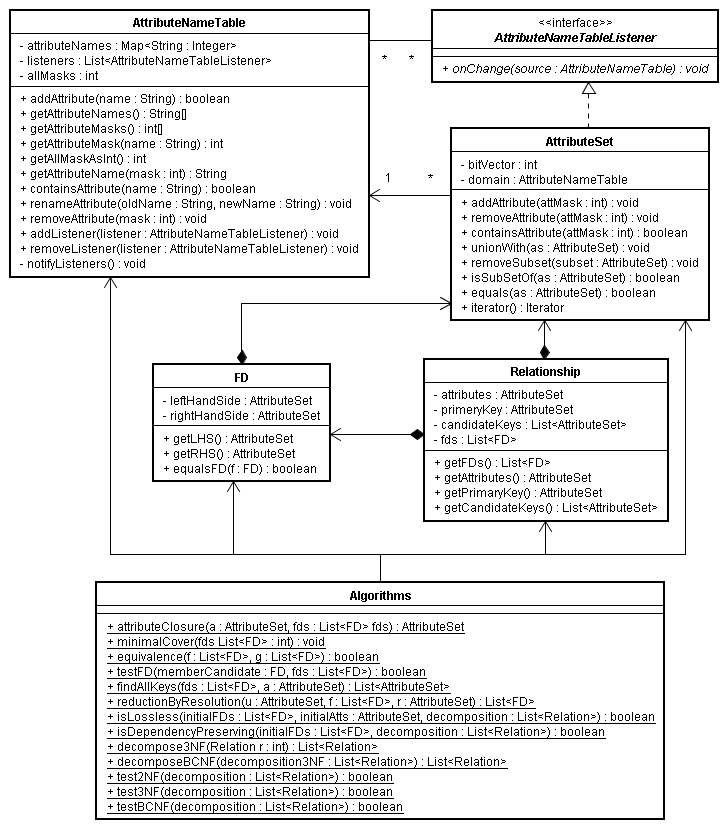
\includegraphics[width=1.08\textwidth]{./img/uml-std.png}
%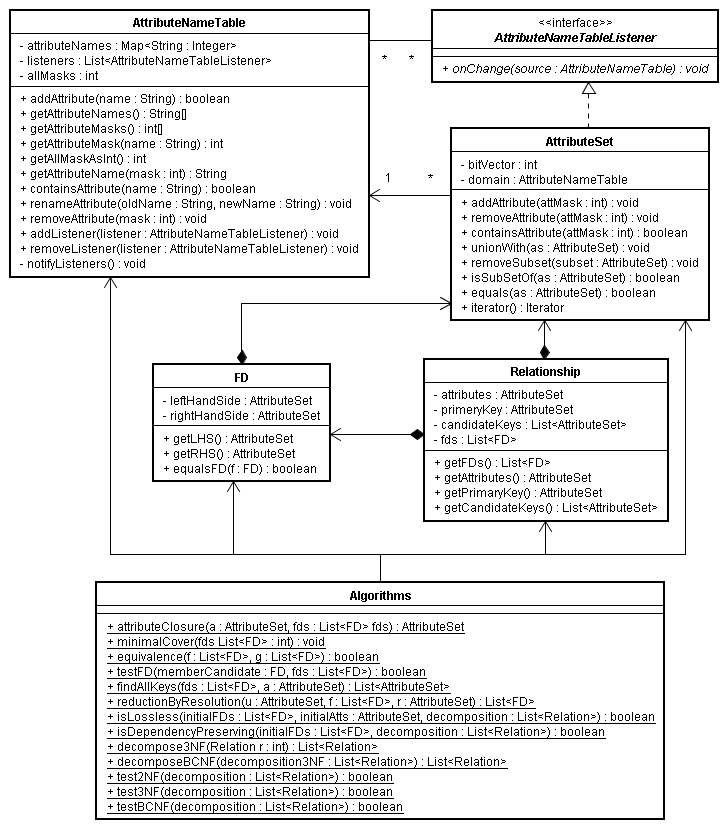
\includegraphics[width=1.00\textwidth]{./img/uml-std.png}
    \caption{LDBN - Core Classes}
    \label{fig:coreuml}
  \end{center}
\end{figure}

%%%%%%%%%%%%%%%%%%%%%%%%%%%%%%%%%%%
% Algorithms                      %
%%%%%%%%%%%%%%%%%%%%%%%%%%%%%%%%%%%
\section{Normalization Algorithms}
\label{sec:alg}
In this section we present different normalization algorithms which are used
in LDBN. A proof of their correctness and complexity would be out of the 
scope of this report and therefore it is omitted. We provide the
reader with textual description and/or pseudo code for each algorithm. 
A reference to additional information is also given. However, in this section we do not
illustrate how the algorithms are applied in the learning environment in order
to perform the \textit{Solve Assignment} and the \textit{Check Solution} functions.
This is done in Section~\ref{sec:keyfunctions}.

We can divide the normalization algorithms used by LDBN into two different groups:

\begin{enumerate}
  \item \textit{Algorithms for Testing} are used to test whether a relation is satisfying a certain normal form criteria.
  \item \textit{Decomposition Algorithms} are used to automatically decompose a relation into a certain normal form.
\end{enumerate}

\subsection{Algorithms for Testing}
\label{sec:algtest}
As we mention earlier we need algorithms for testing whether a decomposition 
is in 2NF, 3NF and BCNF, since a given schema may have many decompositions into a given normal form. Therefore,
simply computing one such decomposition with the \textit{Decomposition Algorithms} and comparing the student's solution to it is
not satisfactory. 

In this section we introduce algorithms for testing weather a decomposition 
is satisfying the lossless-join property, the
dependency preservation property, the 2NF, 3NF and BCNF properties. 
However, most of these algorithms depend on other, more general
algorithms, which we present first.  

\subsubsection{Attribute Closure}
Let $\alpha$  be a set of attributes. 
We call the set of attributes determined by $\alpha$ under a set $F$ of 
FDs the closure of $\alpha$ under $F$, denoted $\alpha +$. The following algorithm
computes $\alpha+$

\begin{alltt}
INPUT
  \(\alpha\)  : a set of attributes
  \(F\)  : a set of FDs
OUTPUT
  \(\alpha+\) : a complete set of attributes  \(\alpha+\)  with  \(\alpha \rightarrow \alpha+\)
BEGIN
  \(\alpha+ = \alpha\)
  while(No more changes in \(\alpha+\)) do
    foreach FD \(\beta \rightarrow \gamma\) in \(F\) do
      if \(\beta \subseteq \alpha+\) then \(\alpha+ \cup \gamma\)
    return \(\alpha+\)
\end{alltt} 

The \textit{Attribute Closure} algorithm is one of the most important algorithms used in LDBN. It is
part of every other normalization algorithm in the system. Therefore every improvement 
of the algorithm is significant. 
The above algorithm is described in many textbooks including~\cite{bdb1, bdb2, bdb4}.
It has worst case behavior quadratic in the size of $F$ and
it is not suitable for large application like LDBN. We presented it only because it is
easy to follow. In our learning environment we use a linear but more complicated algorithm for computing $\alpha+$ 
called $SL_{FD}-Closure$~\cite{p10}:

\begin{alltt}
INPUT
  \(\alpha\)  : a set of attributes
  \(F\)  : a set of FDs
OUTPUT
  \(\alpha+\) : a complete set of attributes  \(\alpha+\)  with  \(\alpha \rightarrow \alpha+\)
BEGIN
  \(\alpha\sb{new} = \alpha\)
  \(\alpha\sb{old} = \alpha\)
  repeat
    foreach FD \(\beta \rightarrow \gamma\) in \(F\) do
      if \(\beta \subseteq \alpha\sb{new}\) then 
        \(\alpha\sb{new} \cup \gamma\)
        \(F = F - \{\beta \rightarrow \gamma\}\) 
      elsif \(\gamma \subseteq \alpha\sb{new}\) then
        \(F = F - \{\beta \rightarrow \gamma\}\) 
      else
        \(F = F - \{\beta \rightarrow \gamma\}\) 
        \(F = F \cup \{\beta-\alpha\sb{new} \rightarrow \gamma-\alpha\sb{new}\}\) 
      end if
    end foreach 
  until ((\(\alpha\sb{new} = \alpha\sb{old}\)) or \(|F| = 0\))
  return \(\alpha+ = \alpha\sb{new}\)
\end{alltt} 

There are several direct uses of the \textit{Attribute Closure} algorithm~\cite{bdb4}:
\begin{description}
    \item[Superkey Test:] To test whether $\alpha$ is a superkey, we compute $\alpha+$, and check whether $\alpha+$ contains all attributes of $R$.
    \item[Computing F+:] For each $\gamma \subseteq R$ we find the closure $\gamma+$, and for each $S \subseteq \gamma+$, we output a FD $\gamma \rightarrow S$.
\end{description}

\subsubsection{FD Test}
To check whether a functional dependency $\alpha \rightarrow \beta $ 
holds (i.e. is in $F+$), just check whether $\beta \subseteq \alpha+$ holds~\cite{bdb4}.
 
\begin{alltt}
INPUT 
  \(f\) : a FD of the form \(\alpha \rightarrow \beta\)
  \(F\) : a set of FDs
OUTPUT 
  true if \(f \in F+\), false otherwise
BEGIN
  compute \(\alpha+ = AttributeClosure(\alpha, F)\)   
  if \(\beta \in \alpha+\) then
    return true
  else
    return false
\end{alltt}
  
\subsubsection{Equivalence}
To determine whether two set of FDs $F$ and $G$ are equivalent, we need to prove that $F+ = G+$. 
However, computing $F+$ or
$G+$ is exponential, therefore this approach cannot be recommended for practical use.
Fortunately, there is a much faster algorithm. We can conclude that $F$ and $G$ are
equivalent, if we can prove that all FDs in $F$ can be inferred from the set of FDs in $G$ and vice
versa. To achieve this we use the \textit{FD Test} algorithm.

\begin{alltt}
INPUT 
  \(F\) : a set of FDs
  \(G\) : a set of FDs
OUTPUT 
  true if \(F \equiv G\), false otherwise
BEGIN
  foreach FD \(f : \alpha \rightarrow \beta\) in \(F\) do
    if not \(FDTest(f, G\)) then
      return false
  end foreach
  
  foreach FD \(g : \alpha \rightarrow \beta\) in \(G\) do
    if not \(FDTest(g, F\)) then
      return false
  end foreach
  
  return true
\end{alltt}

\subsubsection{Lossless-Join Property Test}
In Section~\ref{sec:decofrel} it was shown that a decomposition of $R$ into $R_1$ and $R_2$ 
has a lossless-join if one of the following FDs is in $F+$
\begin{itemize}
  \item $f : R_1 \cap R_2 \rightarrow R_1$ 
  \item $g : R_1 \cap R_2 \rightarrow R_2$ 
\end{itemize}

We can use the \textit{FD Check} algorithm to test whether $f$ or $g$ are in $F+$. Furthermore,
in~\cite{bdb2}, Section~6.5.1, it has been shown inductively that the above rule can be applied for a 
decomposition with $n$ subschemas by using the associativity of the natural join~($\Join$):
$$
  R_1 \Join (R_2 \Join (...\Join(R_{n-1} \Join R_{n}) \newline
  =R_1 \Join (R_2 \Join (...\Join(R_{n-2} \Join R_{n-1}')  \newline
  =
  ...
  = R
$$
Knowing these facts, we can now define a simple algorithm for testing the lossless-join
property of a decomposition \(\mathcal{R}\):
   
\begin{alltt}
INPUT 
  \(R\) : a relation
  \(F\) : a set of FDs which hold in \(R\)
  \(\mathcal{R}\) : a set of relations representing a decomposition of \(R\).
OUTPUT 
  true if  \(\mathcal{R}\) is lossless-join, false otherwise
BEGIN
  K = first element of \(\mathcal{R}\)
  foreach \(R\sb{i} \in \mathcal{R}\) for \(i \geq 2\) do
    if \(FDCheck(K \cap R\sb{i} \rightarrow K, F)\) or \(FDCheck(K \cap R\sb{i} \rightarrow R\sb{i}, F)\) then
      \(K = K \cup R\sb{i}\)
    else
      return false
    end if
  end foreach
  return true
\end{alltt}

%In the above algorithm we are using the $\cup$ operator instead of $\Join$. This is
%permitted, since we are using only the attributes of the relation $R$ and not actual instances (i.e.,
%relation with its contents).

\subsubsection{Dependency Preservation Test} 
Using the \textit{Equivalence} algorithm testing whether a decomposition $R_1,...,R_n$ of $R$ is dependency preserving
becomes quite an easy task. We just need to compute: $$Equivalence(F, (F_1 \cup ... \cup F_n)) \mbox{ where } F_i \mbox{ is the set of FDs which holds in } R_i$$ 

\subsubsection{Find All Candidate Keys}
The problem of finding all candidate keys is know to be NP-complete~\cite{p3}. 
Our leaning environment uses an trivial algorithm for finding all the candidate keys,
which is based on the \textit{Attribute Closure} algorithm. The algorithm test every possible
subset of attributes of the relation for being a superkey. If a subset of the superkey
is found which is also a superkey, then the first superkey is replace with the new one.   

\begin{alltt}
INPUT 
  \(R\) : a relation
  \(F\) : a set of FDs which hold in \(R\)
OUTPUT 
  \(\mathcal{K}\) : a set of all candidate keys for \(R\)
BEGIN
  \(\mathcal{K} = \emptyset\)
  foreach subset \(\gamma\) of \(R\) do
    compute \(\gamma+\)
    if \(\gamma+ \) contains all attributes of \(R\) then
      remove all \(\kappa \in \mathcal{K}\) with  \(\gamma \subseteq \kappa\)
      if \(\gamma \nsubseteq \kappa\) for all \(\kappa \in \mathcal{K}\) then
        \(\mathcal{K} \cup \gamma\)
      end if
    end if
  end foreach
return \(\mathcal{K}\)
\end{alltt}

\subsubsection{Reduction By Resolution}
Often is required to compute a cover for the projection of $F$ on a subschema $X$ of $R$, in 
other words, to find find the FDs on $R$ which are induced by $F$. Altought the problem of
finding such embedded cover of FDs is
known to be inherently exponential~\cite{p11}, it plays an important part of many of the algorithms
used by LDBN. The traditional approach is to compute $F+$ and then project $F+$ over the subschema $X$,
however, the produced cover
is always unnecessarily large~\cite{p4}. Still, for this difficult problem a simple 
algorithm called \textit{Reduction by Resolution}
was found by Gottlob~\cite{p4}. The algorithm is much more practical than the standard approach,
as it runs in polynomial time in a large number of cases, unlike the standard approach
which is exponential for each input. 

\begin{alltt}
INPUT 
  \(R\) : a relation
  \(F\) : a set of FDs which hold in \(R\)
  \(X\) : a subset of attributes of \(R\)
OUTPUT 
  \(F\sb{X}\) : a cover for \(F\sb{X}+\) with 
           \(F\sb{X}+ = \{\alpha\rightarrow\beta | \alpha \rightarrow \beta \in F+ \wedge \alpha \subseteq R \wedge \beta \subseteq R\}\)
BEGIN 
  \(G = F\)
  \(K = X - R\)
  while \(K \neq \emptyset\) do
    choose an element \(A \in K\),
    \(K = K - A\),
    \(RES = \emptyset\)
    foreach FD \(f\) in \(F\) of the form \(Y \rightarrow A\) do
      foreach FD \(g\) in \(G\) of the form \(AZ \rightarrow B\) do
        \(h = YZ \rightarrow B\),
        /* h is the resolvent of f and g */
        if h not trivial then \(RES = RES \cup \{h\}\)
      end foreach
    end foreach
    foreach FD \(f\) in \(G\) do
      if \(A\) occurs in \(f\) then \(G = G - \{f\}\)
    end foreach
    \(G = G \cup RES\)
  end while
  return \(G\)
\end{alltt}

\subsubsection{BCNF Test}
To check whether a non-trivial dependency $\alpha \rightarrow \beta$  causes a violation of BCNF,
we must use the \textit{Attribute Closure} to test whether $\alpha$ is a superkey. 
It suffices to check only the dependencies in the given set $F$ for violation of BCNF, 
rather than checking all dependencies in $F+$~\cite{bdb4}.  
If none of the dependencies in $F$ causes a violation of BCNF, 
then none of the dependencies in $F+$ will cause a violation of BCNF either.
However, using only $F$ is incorrect when testing a relation in a decomposition of $R$~\cite{bdb4}.
Let us consider the following example:

\begin{center}
\begin{tabular}[h]{l l}
  $R = \{A, B, C, D, E\}$ & $F = \{A \rightarrow B, BC \rightarrow D\}$ \\
  Decompose $R$ in:  & $R_1 = \{A, B\} \mbox{ and } R_2 = \{A, C, D, E\}$ \\ 
\end{tabular}
\end{center}

Neither of the dependencies in $F$ contain only attributes from
$(A,C,D,E)$ so we might be mislead into thinking $R_2$ satisfies BCNF. In fact, 
dependency $AC \rightarrow D$ in $F+$ shows $R_2$ is not in BCNF. To avoid this we can
use the \textit{Reduction by Resolution} algorithm to compute covers for $R_1$ and $R_2$. 

The algorithm uses the \textit{Reduction by Resolution} algorithm which is know to be exponential
in some bad cases, thus the \textit{BCNF Test} is also exponential. In fact, the test is know to 
be co-NP-complete~\cite{p4}.

\subsubsection{3NF Test}
The \textit{3NF Test} is similar to the \textit{BCNF Test}. By using the \textit{Reduction by Resolution} algorithm
we must first compute the
embedded FD cover $F_i$ for each relation $R_i$ in a decomposition $R_1,...,R_n$ of $R$. Then we use 
the \textit{Attribute Closure} to test each FD in $F_i$ of the form $\alpha \rightarrow \beta$ 
whether $\alpha$ is a superkey in $R_i$. 
If the $\alpha$ is not a superkey, we have to verify whether each attribute in the $\beta$ 
is contained in a candidate key of $R$, i.e., it is prime. Testing attribute for being a prime
attribute is know to be a NP-complete problem~\cite{p3}. For this part of the \textit{3NF Test} algorithm
we can use our \textit{Find All Candidate Keys} algorithm in order
to compute all the candidate keys in $R_i$ and then test whether the attributes in $\alpha$ are part of any 
of them.

\subsubsection{2NF Test}
%Testing whether a a decomposition is in 2NF is even harder than the \textit{3NF Test}. 
Once again we compute the
embedded FD cover for each relation $R_i$ in a decomposition $R_1,...,R_n$ of $R$. After that 
we compute each candidate key for each for each a relation $R_i$, we refer to this set as $K_i$.
 
To test whether $R_i$ is in 2NF we have to ensure that each non-key attribute is fully
functional dependent on every candidate key in $K_i$. To simply the problem we can test
each FD in $F_i$ of the form $\alpha \rightarrow \beta$ whether $\alpha$ is a proper subset
of a key candidate in $K_i$. If this is true and the attributes in $\beta$ are not prime then
$R_i$ is not in 2NF.

The \textit{2NF Test} is NP-complete, since it involves finding all candidate keys.

\subsection{Decomposition Algorithms}
\label{sec:algdec}
In previous sections we already decomposed some relations without
a formal definition of the rules which we were following during this process. 
In this section we present algorithms for finding a minimal cover of a set of FDs and 
for decomposing any proposed relation into 3NF and BCNF.  

\subsubsection{Find Minimal Cover}
With the help of the \textit{Attribute Closure} algorithm we can now define an algorithm 
for computing a minimal (canonical) cover of a set $F$ of FDs. The algorithm comes form~\cite{bdb2}, Section~6.3.1.

\begin{alltt}
INPUT 
  \(F\)  : a set of FDs
OUTPUT 
  \(F\sb{c}\) : a minimal (canonical) cover of \(F\)
BEGIN

\(F\sb{c} = F\)
repeat
  /* Find redundant attributes in the left-hand side of each FD */
  foreach FD \(\alpha \rightarrow \beta\) in \(F\sb{c}\) do
    foreach \(A \in \alpha\) do
      /* Checks if A is redundant */
      if \(\beta \subseteq AttributeClosure(F\sb{c}, \alpha-A)\) then
        replace \(\alpha \rightarrow \beta\) with \((\alpha-A) \rightarrow \beta\)
      end if
    end foreach
  end foreach
    
  /* Find redundant attributes in the right-hand side of each FD */
  foreach FD \(\alpha \rightarrow \beta\) in \(F\sb{c}\) do
    foreach \(B \in \beta\) do
      /* Checks if B is redundant */
      if \(B \subseteq AttributeClosure(F\sb{c}-(\alpha \rightarrow \beta) \cup (\alpha \rightarrow (\beta - B)), \alpha)\) then
        replace \(\alpha \rightarrow \beta\) with \((\alpha \rightarrow (\beta-B)\)
      end if
    end foreach
  end foreach
    
  Delete all FDs FD of the form \(\alpha \rightarrow \emptyset\) form \(F\sb{c}\)
    
  Using the \(Union Rule\) combine all FDs of the form \(\alpha \rightarrow \beta,...,\alpha \rightarrow \gamma\)
    into one FD \(\alpha \rightarrow (\beta \cup ... \cup \gamma)\)
    
until \(F\sb{c}\) does not change
return \(F\sb{c}\)
\end{alltt}

For the sake of simplicity we iterate over all FDs in $F$ several times, in the actual implementation
the number of iteration could be reduced. 

\subsubsection{3NF Decomposition}
The following algorithm decomposes a relation schema in 3NF. The algorithm
ensures that each new relation schema is in 3NF, thus the decomposition is in 3NF. 
Furthermore, the decomposition is dependency preserving and lossless-join. 
The algorithm comes form~\cite{bdb2}, Section~6.8. 
First, we build new relations corresponding to each FD in in $F_{c}$ (the minimal cover of $F$). 
Then we need to eliminate relations, the attributes of
which are subset of the attributes of another relation. 
After that, we find all the candidate keys of
the initial relation, this is necessary in order to determine  whether one of them is present
in the new set of relations, which is required by the algorithm to ensure
dependency preservation. If this is not the case, the algorithm creates
a new relation \(\mathcal{R}\sb{i}\) = any candidate key for \(R\).
Here follows a pseudo code of the algorithm:

\begin{alltt}
INPUT 
  \(R\)  : a relation
  \(F\sb{c}\) : a canonical cover of a set of FDs which hold in \(R\)
OUTPUT 
  \(\mathcal{R}\) : a set of relational schemas representing a decomposition in 3NF 
BEGIN
  \(\mathcal{R} = \emptyset\)
  i = 0
  foreach FD \(\alpha \rightarrow \beta\) in \(F\sb{c}\) do
    i = i + 1
    create a relation schema \(\mathcal{R}\sb{i} = \alpha \cup \beta\)
    assign \(\mathcal{R}\sb{i}\) the FDs  \(F\sb{i} = \{\alpha\sp{'} \rightarrow \beta\sp{'} \in F\sb{c}\ | \alpha\sp{'} \cup \beta\sp{'} \subseteq \mathcal{R}\sb{i}\}\)
    \(\mathcal{R} = \mathcal{R} \cup \mathcal{R}\sb{i}\)
  end foreach
  
  if none of the schemas \(\mathcal{R}\sb{j}, 1 \leq j \leq i\) contains a candidate key for \(R\) then
    i = i + 1
    create a relation schema \(\mathcal{R}\sb{i}\) = any candidate key for \(R\)
    \(\mathcal{R} = \mathcal{R} \cup \mathcal{R}\sb{i}\)
    
  Delete all relational schemas \(\mathcal{R}\sb{a}\) from \(\mathcal{R}\) with \(\mathcal{R}\sb{a} \subseteq \mathcal{R}\sb{j},  1 \leq j \leq i\)
  
  return \(\mathcal{R}\)
\end{alltt}

\subsubsection{BCNF Decomposition}
There is a simple algorithm for decomposing a relational schema into BCNF.
It is described in~\cite{bdb2}, Section~6.9:

\begin{alltt}
INPUT
  \(R\) : a relation
  \(F\) : a set of FDs which hold in \(R\)
OUTPUT
  \(Z\) : a set of relational schemas representing a decomposition in BCNF 
BEGIN
\(Z = R\)
done = false

while not done do
  if there is a schema \(R\sb{i}\) in \(Z\)  that is not in BCNF then begin
    let \(\alpha \rightarrow \beta\) be a nontrivial FD that holds on \(R\sb{i}\)
      such that \(\alpha \nrightarrow R\sb{i}\) /* \(\alpha\) is not a superkey */
      and  \(\alpha \cap \beta \neq \emptyset\) then  
        decompose \(R\sb{i}\) in \(R\sb{i1} = \alpha \cup \beta\) and \(R\sb{i2} = R\sb{i} - \beta\)
        remove \(R\sb{i}\) from \(Z\) 
        \(Z = Z \cup R\sb{i1} \cup R\sb{i2}\)
  else 
    done = true
  end if 
return \(Z\)
\end{alltt}

The algorithm always 
procures a lossless-join decomposition, however, we must run the \textit{Dependency Preservation Test} on
the decomposition to check whether the decomposition is dependency preserving or not. As we mention in Section~\ref{sec:BCNF},
it is no always possible to find a dependency preserving BCNF decomposition.



\section{Key Functions of LDBN}
\label{sec:keyfunctions}
As we stated earlier, the two most important functions of LDBN are the \textit{Solve Assignment} and 
the \textit{Check Solution} functions. They build the foundation of the system and
without them UI will lose its purpose. Therefore, we
discuss the two function more formally in this section.

\subsubsection{Solve Assignment}  
The \textit{Solve Assignment} function can provide the user with a sample solution
to an assignment, thus it decomposes a database schema from URF into 3NF and BCNF. This
task involves several algorithms. Figure~\ref{fig:orderdecomposition} is 
illustrates the order in which those algorithms are applied.

\begin{figure}[h]
	\begin{center}
		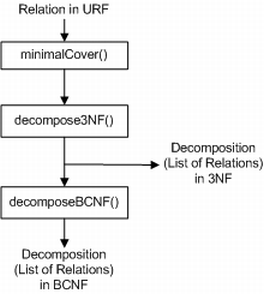
\includegraphics[scale=0.6]{./img/decomposition1a.png}
		\caption{Order of the Decomposition Algorithms}
		\label{fig:orderdecomposition}
	\end{center}
\end{figure}

First, the schema is passed trough the
\verb=minimalCover()= method of the \verb=Algorithms= class, which
implements the Algorithm \textit{FindMinimalCover} of Figure~\ref{alg:mincov}. 
After that we use the \verb=decompose3NF()= method, which implements the 
decomposition algorithm described in Figure~\ref{alg:dec3nf}. 
We use the new decomposition also as a solution for the 2NF, since
a decomposition in 3NF is also in 2NF. 

For computing the BCNF decomposition we use 
a slight modification of the Algorithm \textit{DecompositionBCNF} of Figure~\ref{alg:decbcnf}.
In our implementation
the input for the algorithm is not the initial schema in URF, but the decomposition
produced by the \verb=decompose3NF()= method. By doing this we 
increase the performance of the system, since many decompositions which 
are in 3NF are also in BCNF, or the differences are usually rather small, thus the algorithm
requires fewer passes.   
  
A given schema will always have a dependency-preserving 3NF
decomposition, as well as a BCNF decomposition, but not necessarily a
dependency-preserving BCNF decomposition. Thus, there are two
distinct final goals for decomposition which may not always be
realizable simultaneously. Because of this fact, we do not present the BCNF decomposition as solution
for the 3NF, even though BCNF decompositions are also in 3NF.

\subsubsection{Check Solution}  
The \textit{Check Solution} function of LDBN allows the system to test a solution 
provided by the user and assess its correctness relative to many factors, which
we present later in this section. As we mentioned earlier it is not possible
to compare a solution produces by LDBN to the one of the user, since there may be many
possible solutions/decompositions to a given database schema. Therefore we need the
algorithms for testing a decomposition described in Section~\ref{sec:algtest}. In this section
we illustrate how we apply those algorithms in our implementation. 

First of all, a solution in LDBN is represented as a list of instances of the
\verb=Relation= class. Those objects are built from the user input. The list is then
passed to the static functions in the \verb=Algorithm= class, which 
implement the all of the algorithms described in Section~\ref{sec:alg}. 
The system analyzes the solution to the following factors:

\begin{description}
  \item [Correctness of the FDs] of each relation, this means, testing whether the FDs associated by the user
    for each new relation are actually in the closure of FDs for this relation. We do this by
    using the Algorithm \textit{ReductionByResolution} of Figure~\ref{alg:rbr} for computing the embedded closure of FDs for the given
    relation. This algorithm is implemented by the \verb=reductionByResolution()= method. Then we apply
    the \textit{Equivalence} algorithm of Figute~\ref{alg:equivalence}, to test 
    whether both set of FDs, the one produced by 
    the algorithm and the one provided by the user, are equivalent. Here the Algorithm \textit{ReductionByResolution}
    can have exponential complexity in some bad cases~\cite{p4}, therefore we cache the results
    of the algorithm for future use, e.g., when the user needs to recheck his solution, which can happen
    quite often during the process of solving an assignment correctly. 

	\item [The Losses Join] properly for every decomposition. This check is done by directly applying the 
		Algorithm \textit{TestLosslessJoin} of Figure~\ref{alg:lossless}, which is 
		implemented by the \verb=isLossless()= method.
		
	\item [Dependency Preservation] for every decomposition. This check is done by directly applying the 
		Algorithm \textit{TestDependencyPreservation} of Figure~\ref{fig:dptest}, which is implemented by the 
		\verb=isDependencyPreserving()= method.
		
	\item [Correctness of the Key] of each relation. This check is performed by first computing 
		every possible candidate key 
		for each new relation, by applying the Algorithm \textit{FindAllCandidateKeys} of Figure~\ref{alg:findkeys}, 
		which is implemented
		by the \verb=findAllKeys()= method. The method returns a list of all possible candidate keys
		for a given relation. Then the system searches if the key suggested by the user is 
		present in that list. The algorithm is quite slow due to the fact that the problem of
		finding all candidate keys is know to be NP-complete~\cite{p3}. To improve performance LDBN
		caches every list found for each relation, so that whenever a user needs to rechecks his/her solution
		the system computes only the lists of candidate keys for new, uncached relations.  
		
	\item [Correctness of the Decomposition] In this check we apply directly the 
		\textit{Test2NF, Test3NF, Test BCNF}, which are implemented by the 
		\verb=test2NF()=, \verb=test3NF()=, \verb=testBCNF()= methods.
\end{description}

All the checks are performed in the exact order described above. If one of the checks fails the following ones
are not executed. This way we are able to give the user faster feedback, because 
the most computationally expensive checks are at the end. For example, if the \textit{Dependency Preservation}
check, which is performed in polynomial time, fails, then the other check such as the 
\textit{Correctness of the Key} and the \textit{Correctness of the Decomposition}, both of which 
have exponential complexity, are omitted, thus the user could get a much faster response from the system
in case of an error. 

\section{User Interface}
The most important part of a system for end users and critical for system 
success is the user interface (UI)~\cite{p9}, as such we put most of
our efforts in developing a fast, intuitive and stable UI. Furthermore,
it is possible to define two distinct user groups, warranting at least two different
user interfaces for LDBN.  One group would include the lecturers, who will
focus their attention on creating assignments. The other group would be the 
students, who will use the leaning environment mostly for solving 
the assignments provided by the lecturers. It should be noted that every registered
user can create assignments, thus students can take the role of lecturers as well.
We tried to provide both 
user groups with fast and easy to use UI. In order to achieve this we put a lot
of our attention in finding a good layout for the UI. The requirements for
the layout were to give the user as much information possible about an 
assignment without losing the general view. In order to achieve this goal  
we split the UI in four different views using tabs:

\begin{description}
	\item[Home] view is where the users can login, register and view some information 
	about the learning environment. It can be seen in Figure~\ref{fig:hv}.
	\item[Solve Assignment] view is where students can load an assignment, give and
	test their solutions. In case they have troubles finding a correct solution
	LDBN could generate a sample one and present it. Figure~\ref{fig:sav} is showing
	the view with a loaded assignment.
	\item[Create Assignment] view is used by lecturers to create, edit, export or import
	assignments. It can be seen in Figure~\ref{fig:cav}.
	\item[License] view displays a license information about LDBN.
\end{description} 

\begin{figure}[h]
	\begin{center}
		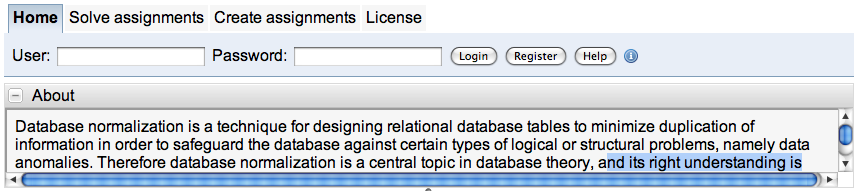
\includegraphics[width=0.85\textwidth]{./img/screen-tab1.png}
		\caption{Home View}
		\label{fig:hv}
	\end{center}
\end{figure}

\begin{figure}[h]
	\begin{center}
		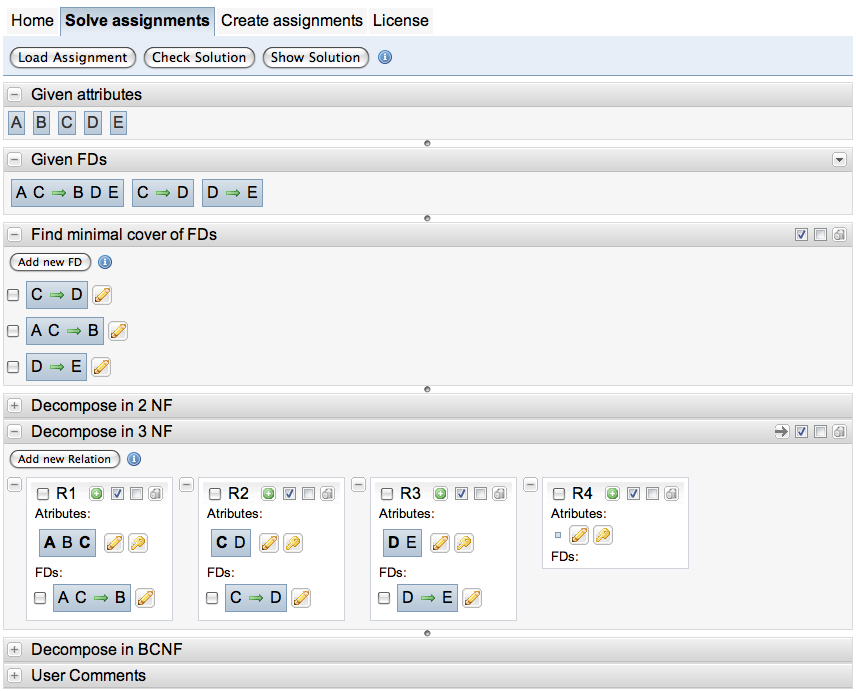
\includegraphics[width=0.85\textwidth]{./img/screen-tab2.png}
		\caption{Solve Assignments View}
		\label{fig:sav}
	\end{center}
\end{figure}

\begin{figure}[h]
	\begin{center}
		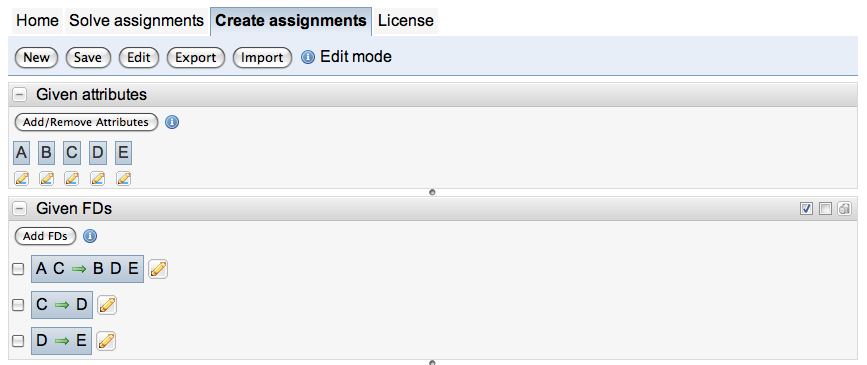
\includegraphics[width=0.85\textwidth]{./img/screen-tab3.png}
		\caption{Create Assignments View}
		\label{fig:cav}
	\end{center}
\end{figure}


\subsubsection{Solve Assignment View}
The most important view for students is definitely the \textit{Solve Assignment} view.
It contains the following fields:

\begin{itemize}
	\item Given attributes.
	\item Given FDs.
	\item Minimal Cover.
	\item 2NF, 3NF, BCNF Decomposition.
	\item Comments.
\end{itemize}

The \textit{Given Attitibutes} and the \textit{Given FDs} fields are not editable
and they correspond	to the information stored in each assignment, which is all the 
attributes and all the FDs of a database schema in URF. In all other fields 
the content can be modified by the user using different editors,
such as the \textit{Attribute Editor} (Figure~\ref{fig:attedit}), 
the \textit{Key Editor} (Figure~\ref{fig:keyedit}) and the \textit{FD Editor}
(Figure~\ref{fig:fdedit}).
All of those editors contain one or two text boxes, where users can input 
different attribute names separated by commas
in order to define respectively attributes of a relation, a key or a set of FDs. With
the help of the editors the user can define relations like the one shown on 
Figure~\ref{fig:relui}. In this example we have a relation with attributes 
\textit{\{A, B, C\}}, a key \textit{\{A, C\}} and only one FD in the set of FDs,
namely \textit{\{A, B $\rightarrow$ C\}}.  Furthermore,
each of the editors is wrapped in a draggable dialog window. 
In this way, the editors do not require any space on any of the fields, 
and can be opened only when they are needed. In addition to this, every attribute and every FD,
like the ones shown in the relation on Figure~\ref{fig:relui}, can be dragged and
dropped in the text box of each editor, as a result of which the attributes/FDs
are automatically inserted in the text areas of the editor.
This can help user define attributes, keys or
FDs much more quickly, which on the other hand can help improve the usability of 
the learning environment. 

\begin{figure}[h]
	\centering
	\subfigure[Attribute Editor]{
		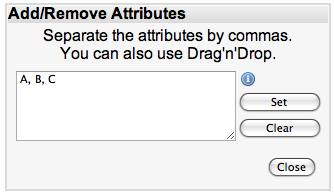
\includegraphics[scale=0.4]{./img/screen-atteditor.png}
		\label{fig:attedit}
	}
	\subfigure[Key Editor]{
		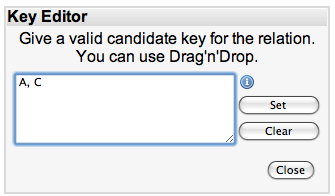
\includegraphics[scale=0.4]{./img/screen-keyeditor.png}
		\label{fig:keyedit}
	}
\caption{Attribute and Key Editor}
\end{figure}

\begin{figure}[h]
	\centering
	\subfigure[FD Editor]{
		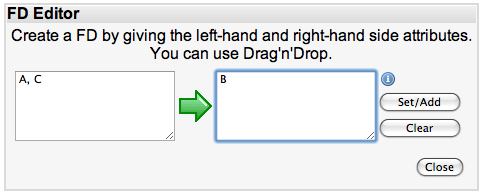
\includegraphics[scale=0.4]{./img/screen-fdeditor.png}
		\label{fig:fdedit}
	}
	\subfigure[Relation]{
		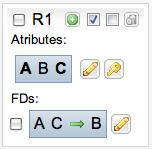
\includegraphics[scale=0.52]{./img/screen-rel.png}
		\label{fig:relui}
	}
\caption{FD Editor and an Example of a Relation in LDBN}
\end{figure}

We continue with the different fields in \textit{Solve Assignment} view. 
The first one is the \textit{Minimal Cover} field, where the user has to define 
a set of FDs using the \textit{FD Editor}. The user defined FDs must
constitute a minimal cover of the \textit{Given FDs}.
This field is intended to be an intermediate step, which will help the user 
find easier a correct decomposition
in the \textit{2NF, 3NF and BCNF Decomposition} fields. Those last three fields all
work the same way, with the only difference that the alogotithms for checking the 
correnctnes of the 
decomposition are not the same.  
In each decomposition field the user must define a set of relations, like the one shown 
in Figure~\ref{fig:relui}. All the relations
within a field represent a decomposition. To check the decomposition the user must
use the \textit{Check Solution} button, 
after that the system analyzes the solution by the criteria described in 
Section~\ref{sec:keyfunctions} and shows a dialog with the result 
as the one in Figure~\ref{fig:screen03} 

Another useful feature, which also improves the usability of LDBN and greatly reduces
the time for defining relations, 
is the ability to 
import entire decompositions from the 2NF into the 3NF field, and from the 
3NF field into the BCNF field. This was done because usually 
the differences between the decompositions are not huge, and each decomposition
can be used as a good staring point for the other ones.	

The last field of the \textit{Solve Assignemtn} view is the \textit{Comment} field, 
where users can view and post textual comments on every assignment.

\subsubsection{Create Assignment View}
The \textit{Create Assignment} view looks very similar to the 
\textit{Solve Assignment} view. It also has a \textit{Given Attributes} and 
\textit{Given FDs} fields. However, in this view these fields
can be edited using the \textit{Attribute Editor} and the \textit{FD Editor}. 
This allows users to define new assignments or modify existing ones. In addition, the view
allows users to save the assignments in the database or to export them as XML
files to the local file system. Importing an assignment form an XML file is also 
possible.  
\newline
Finally, in case the user needs any help with certain aspects of LDBN, the system provides 
help dialogs for every key feature of the UI. The dialogs can be open
using information buttons (
\includegraphics[scale=0.5]{./img/info.png}), which can be
found near every button or in every editor. This way help information is 
visually organized and the user has fast access to it. An example of such help dialog
window is shown in Figure~\ref{fig:screen-help}.

\begin{figure}[h]
	\begin{center}
		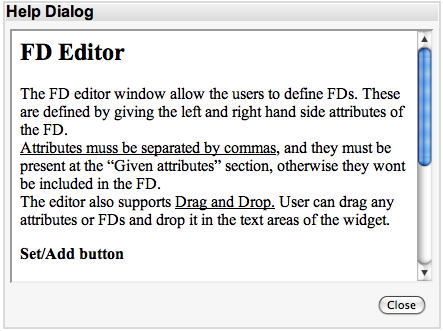
\includegraphics[width=0.5\textwidth]{./img/screen-help.png}
		\caption{Help Dialog for the FD Editor}
		\label{fig:screen-help}
	\end{center}
\end{figure}


\section{Server Side}
The server side is mainly used for persistent storage of assignments, user comments,
user and session data. The communication between the web server and the client
is done using the POST method of the Hypertext Transfer Protocol - HTTP/1.1~\cite{w6}.
The POST method has two advantages over the GET method. First, it is more secure, i.e., 
the GET method is defined as safe, which means it is intended only for information 
retrieval and should not change the state of the server. Second, although the
RFC 2616, "Hypertext Transfer Protocol -- HTTP/1.1"~\cite{w6} does not specify
any requirement for URL length, many browsers like Internet Explorer limit
the length of an URL to a maximum of 2048 characters. This length may not be 
enough for LDBN, as it sometimes sends very large assignments back to the server.  

The web server uses XML to send data back to the client. LDBN defines its own XML data
exchange format. The format has several types:

\begin{description}
	\item[Message] for sending string messages, which appear in an alert window on 
	the client side. Such messages can be for instance an error messages returned
	by the database. 
	\item[Comments] for sending user comments. 
	\item[Session] contains session data for logged in users such as a unique session 
	ID, generated by the server and stored in the database. The ID is used for
	authorizing user actions on the server side.
	\item[Assignment List] for sending back meta data for each assignment. This
	information is used by the \textit{Load Assignment} function in order 
	to display a list of all available assignments from the database.
	\item[Assignment] contains a LDBN assignment. 
\end{description}  

\section{Security Issues}
The system uses HTTP 1.1 for the communication between the client and the web
server. This can easily be secured by using HTTPS instead. The upgrade only
require changes to the configuration of the web server. However, using an encrypted
connection does not prevent web applications from SQL injection and cross-site 
scripting attacks. SQL Injection refers to the technique of 
inserting SQL statements into web-based input fields in 
order to manipulate the execution of the SQL queries. Cross Site Scripting 
attacks work by embedding script tags into the web pages. 

Here follows a short example of a SQL injection.
Assuming that we have a poorly implemented PHP script for loading an assignment,
which has the following line of code in it:

\begin{verbatim}
     $sql_statement := "SELECT * FROM assignment WHERE id=$_GET['id'] ";
\end{verbatim}

\noindent If the $id$ argument of the GET method is crafted in a specific way by a 
malicious user, the SQL statement may do more than the code author intended. 
For example, setting the $id$ argument as:

\begin{verbatim}
     1; DROP TABLE users;
\end{verbatim}

\noindent yields the following SQL statement:

\begin{verbatim}
     SELECT * FROM assignment WHERE id=1; DROP TABLE users;
\end{verbatim}

\noindent The statement would cause the deletion of the $users$ table. 

In order to prevent SQL injection and cross-site 
scripting attacks LDBN uses regular expressions for validating
user input, and it escapes HTML special characters like \lt and~\gt.
To the best of our knowledge, it is not possible to perform such attacks on LDBN.

Another issue with web-based applications is password protection. LDBN uses the 
MD5~\cite{w7} one-way encryption algorithm for hashing user passwords. 
To authenticate a user, the password presented by him/her is hashed on the client side, 
then send to the web server and compared to the stored hash in the database. 
This way the actual password of the user is never sent over the network.
